\documentclass[twocolumn]{article}
\usepackage{graphicx}
\usepackage{geometry}
\geometry{margin=1in}
\usepackage{amsmath}
\setlength{\columnsep}{1cm}
\usepackage{listings}
\usepackage{xcolor}
\usepackage{url}
\usepackage{float}
\usepackage{authblk}

\title{Classifying Marine Mammals Using Convolutional Neural Networks}
\author[1]{Aditya Katre}
\author[2]{Arpit Jasapara}
\affil[1]{Del Norte High, San Diego, California}
\affil[2]{University of California Los Angeles, Los Angeles, California}
\begin{document}
\date{December 2024}
\maketitle

\begin{abstract}
Deep learning continues to rapidly advance image recognition capabilities, providing cutting-edge support for wildlife conservation initiatives. In this study, we develop a Convolutional Neural Network (CNN) framework to distinguish individual whales and dolphins extracted from the Happywhale dataset, demonstrating high precision in marine mammal identification. Our model achieves robust feature extraction and enhanced class separability by leveraging an EfficientNetB5 backbone with an ArcFace loss function. Multiple data augmentation techniques, including random cropping, grayscale conversion, and color manipulations, are employed to further strengthen the model’s adaptability across varied imaging conditions. Additionally, a k-nearest neighbors (KNN) algorithm is incorporated at the inference stage to refine predictions, especially for previously unseen images. Through these combined strategies, our final model significantly boosts classification accuracy, achieving a Mean Average Precision at 5 score of 0.88 and showcasing the efficacy of deep learning solutions for fine-grained identification tasks in marine mammal conservation. The promising results highlight the model’s potential for streamlining research workflows and informing long-term conservation strategies for whales, dolphins, and other marine species.
\newline
\newline
Keywords: Marine Mammal Identification, Convolutional Neural Network (CNN), Deep Learning, EfficientNetB5, ArcFace, Data Augmentation, K-Nearest Neighbors (KNN), Wildlife Conservation, MAP@5, Population Tracking
\end{abstract}

\section{Introduction}
Identifying and classifying individual marine mammals is critical for research on marine mammal conservation efforts and population tracking. Traditional identification methods rely heavily on manual photo matching, which is time-consuming and prone to human error. Artificial intelligence and machine learning offer robust ways to automate the identification of marine mammals with high accuracy\textsuperscript{1}.

This research leverages the Happywhale dataset, which includes tens of thousands of labeled images representing fifteen thousand unique marine mammal individuals across 30 distinct species. The goal is to create a model capable of effectively and reliably distinguishing individual animals based on physical features such as fluke shape, skin patterns, and body size. This study leverages a pre-trained EfficientNetB5 backbone as the feature extractor and integrates an ArcFace loss layer to enhance model performance by maximizing the separation between classes (i.e., individuals).

Additionally, this research explores various image augmentation techniques to improve the model's generalization ability. This study demonstrates the potential of deep learning for wildlife monitoring and establishes a practical and scalable framework for similar applications where technology meets biology.

\section{Background}
The Happywhale data set is a whale and dolphin identification challenge consisting of over 51,000 labeled images representing 15,587 unique marine mammals over 30 different species. These images were collected through contributions from marine researchers and photographers supporting the identification, tracking, and conservation of marine mammal populations around the world. Whales and dolphins are typically recognized by their distinct features such as fluke shape, dorsal fin markings, skin patterns, and shape\textsuperscript{2}. However, the difficulty of manually classifying individual images of marine mammals has led to the need for artificial intelligence recognition systems to automate this task. 

Identifying individual whales and dolphins is essential to understanding their populations, social dynamics, and migration routes. These marine mammals exhibit unique physical features, like markings or scars, which can serve as natural identifiers. Traditionally, scientists have collected photographs of these markings and manually matched them to existing records. Although this manual photoidentification method has proven to be effective over the years, it is often time consuming and expensive. As researchers gather larger datasets, the potential for human error increases, making it difficult to maintain accuracy. Additionally, this manual process can create significant delays in data analysis, which can be critical when monitoring the health of marine ecosystems and the effect of environmental changes\textsuperscript{3}. Identifying individuals is challenging due to subtle variations in markings, environmental factors, and image quality, making machine learning models essential for use in the real world.

The primary objective of this study is to develop a model that can accurately and reliably classify individual whales, dolphins, and other marine animals within the Happywhale dataset. This high-performance identification model will support marine biologists and conservationists in tracking marine mammal populations. The approach utilizes modern machine learning techniques, such as transfer learning and data augmentation. These methods allow the model to handle the complexity and unpredictability of real-world images. 

This research fills a critical gap in marine animal conservation by developing an automated and scalable approach to identify individuals. The methods used in this study are designed to achieve high accuracy and provide a practical tool for conservationists, directly contributing to the sustainability and conservation efforts of marine mammals worldwide. 

\section{Methodology}
The methodology of this study is to develop the best possible deep learning model to classify whale and dolphin images into specific categories. The model’s design and training processes were optimized to enhance both accuracy and generalizability, leveraging transfer learning, loss functions, and various techniques for data augmentation. Here are the key components used to set up the model:

The model uses EfficientNetB5 as its backbone. EfficientNetB5 is a convolutional neural network that strikes a balance between accuracy and efficiency, ensuring the model runs promptly while minimally sacrificing accuracy\textsuperscript{4}. The EfficientNetB5 model efficiently scales the neural network across three dimensions: 

\begin{enumerate}
    \item \textbf{Depth Scaling:} This increases the depth of training data, allowing the model to learn subtle patterns in images. This enables the model to learn from more complex, layered data. However, overusing this method may lead to higher computational demands and a decline in efficiency.
    \item \textbf{Width Scaling:} This method of scaling adds more neurons to each layer of the model, expanding its width. As a result, the CNN can learn more nuanced patterns in data. Depth and width scaling work in harmony to effectively extract features from data.
    \item \textbf{Resolution Scaling:} The EfficientNetB5 model scales images in a balanced manner, ensuring that images are high-quality and that nuanced features can be extracted while maintaining a decent level of computational demand.
\end{enumerate}

The ArcFace loss layer is introduced as the classification head for this model. ArcFace increases the separation between different classes, improving the model’s ability to distinguish images. It achieves this by introducing Additive Angular Margin Loss to the feature vectors. This additional margin in ArcFace creates a more robust distinction between image classes. This enhanced the model’s discriminative learning and accuracy in identifying images across a large subset of classes. The loss layer operates by normalizing each feature and then using a cosine similarity metric for each feature. Then, ArcFace makes it easier to distinguish between classes by adding a fixed angle, or angular margin, between the feature vector and target class. This contributes to making class boundaries more distinct, enforcing a distinct separation between classes.\textsuperscript{5}.

\subsection{Architecture Selection Rationale}

Prior to selecting EfficientNetB5 as our backbone architecture, experiments were conducted to compare multiple models on their inferencing capabilities on the Happywhale dataset. Our selection criteria included computational efficiency when using Tensor Processing Units (TPUs), performance on fine-grained image classification tasks, and its ability to process high-resolution images while using maintaining reasonable memory requirements. 

EfficientNetB5 was compared against several baseline architectures, including ResNet50, EfficientNetB3, EfficientNetB5, and EfficientNetB7. The selection of EfficientNetB5 was based on its balance between accuracy and computational cost. Specifically, EfficientNetB5 demonstrated superior feature extraction capabilities and reasonable computational demand compared to other models when tested on the Happywhale dataset.

\subsection{Data Preparation and Augmentation}

Kaggle’s Happywhale dataset is split into training and testing sets. A CSV file containing the filename for each image and the corresponding label for the image is included. Some labels include: \(bottlenose\_dolphin\), \(beluga\), \(killer\_whale\), \(blue\_whale\), and many others. Each image in the training set undergoes a series of transformations to improve the model’s capability to process and develop an understanding of features in the images. The key transformations that the images undergo include:

\begin{itemize}
    \item \textbf{Random Cropping:} Images are cropped randomly using full-body, YOLOv5, Detic, or Vision Transformer. This allows the model to focus on specific body parts of the whale or dolphin.
    \item \textbf{Color Adjustments:} Hue, saturation, contrast, and brightness are randomly altered to allow the model to handle various lighting and color conditions effectively.
    \item \textbf{Grayscale Conversion:} Converting images to grayscale enhances the model’s ability to recognize patterns based solely on pixel intensity values. 
\end{itemize}

\begin{figure}
    \centering
    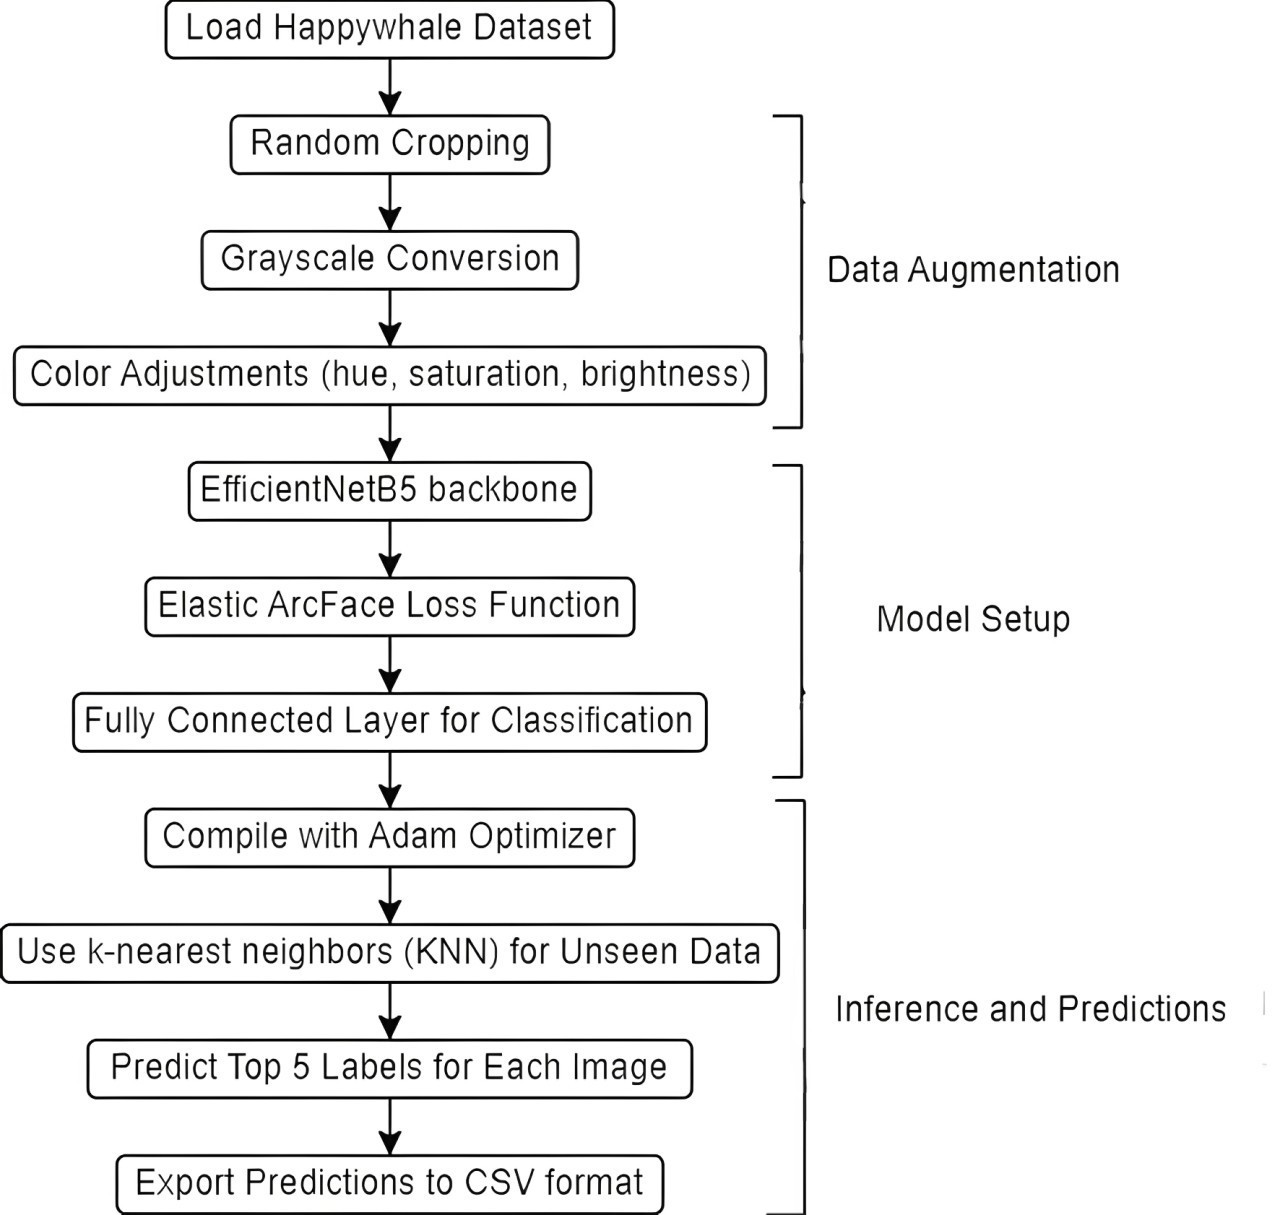
\includegraphics[width=0.7\linewidth]{model3.jpg}
    \caption{Flowchart-style architecture diagram of the EfficientNetB5 model with ArcFace loss function. The flowchart begins by performing image augmentations on training data, creates a model, and finally runs to make predictions, which are exported to a CSV format and submitted.}
\end{figure}

\subsection{Data Splitting and Leakage Prevention}

Kaggle distributes the dataset in two completely separate folders in the Happywhale competition. The first, \texttt{train\_images/}, is accompanied by a \texttt{train.csv} file that lists the species and \texttt{individual_id} for every training photo. The second, \texttt{test_images/}, contains unlabeled images. While some individuals that appear in the test set can be absent in the training data, no image in the training folder is duplicated in the test folder. This organizer-enforced separation and organization of images eliminates the risk of leakage between the two data folders.  

\subsection{Class Imbalance Analysis}

The Happywhale training dataset exhibits severe class imbalance across species, with bottlenose dolphnis representing 9,664 images while species such as Fraser's dolphins contain only 14 images.  Image classes such as the Killer Whale are in the middle of the pack, representing 962 images in the training dataset. 

The species distribution follows a pattern commonly seen in real-world ecological datasets. The top five most common species accounts for 64.7\% of all images, while the bottom 10 species collectively represent less than 3\% of the dataset. Individual-level imbalance is even more pronounced, with some individuals appearing in hundreds of images while others have only single instances. 

\begin{table}[ht]
\centering
\begin{tabular}{l r}
\hline
\textbf{Species} & \textbf{Image Count} \\
\hline
\texttt{bottlenose\_dolphin}           & 9\,664 \\
\texttt{beluga}                        & 7\,443 \\
\texttt{humpback\_whale}               & 7\,392 \\
\texttt{blue\_whale}                   & 4\,830 \\
\texttt{false\_killer\_whale}          & 3\,326 \\
\texttt{dusky\_dolphin}                & 3\,139 \\
\texttt{spinner\_dolphin}              & 1\,700 \\
\texttt{melon\_headed\_whale}          & 1\,689 \\
\texttt{minke\_whale}                  & 1\,608 \\
\texttt{killer\_whale}                 & 1\,493 \\
\texttt{fin\_whale}                    & 1\,324 \\
\texttt{gray\_whale}                   & 1\,123 \\
\texttt{bottlenose\_dolphin}            & 1\,117 \\
\texttt{killer\_whale}                  &   962 \\
\texttt{southern\_right\_whale}        &   866 \\
\texttt{spotted\_dolphin}              &   490 \\
\texttt{sei\_whale}                    &   428 \\
\texttt{short\_finned\_pilot\_whale}   &   367 \\
\texttt{common\_dolphin}               &   347 \\
\texttt{cuviers\_beaked\_whale}        &   341 \\
\texttt{pilot\_whale}                  &   262 \\
\texttt{long\_finned\_pilot\_whale}    &   238 \\
\texttt{white\_sided\_dolphin}         &   229 \\
\texttt{brydes\_whale}                 &   154 \\
\texttt{pantropic\_spotted\_dolphin}   &   145 \\
\texttt{globis}                        &   116 \\
\texttt{commersons\_dolphin}           &    90 \\
\texttt{pygmy\_killer\_whale}          &    76 \\
\texttt{rough\_toothed\_dolphin}       &    60 \\
\texttt{frasers\_dolphin}&    14 \\
\hline
\end{tabular}
\caption{Species distribution within the Happywhale dataset.}
\label{tab:species_counts}
\end{table}

\subsection{Imbalance Mitigation Strategy}

Our approach to handling the severe class imbalance combines several complementary techniques rather than relying on traditional oversampling methods. The implementation addresses imbalances at multiple stages of the model creation pipeline:
\begin{enumerate}
\item Cross-validation Based Data Splitting: We implemented a 10-fold cross-validation strategy that ensures balanced representation across each fold while maintaining the natural distribution within each fold. This approach helps prevent overfitting to overrepresented classes during training and provides more robust performance across groups with different frequencies in the  dataset. 
\item Augmentation-based Minority Class Enhancement: Rather than utilizing traditional oversampling methods, we applied data augmentation techniques, such as random horizontal flipping and other techniques, across all classes. This strategy indirectly benefits minority classes by increasing their effective representation through transformations while preserving biological features critical for species identification.
\item Natural distribution preservation: Maintaining original class distribution during training was feasible because natural encounter frequencies present in the training dataset contain valuable ecological information. Artificially balancing the training dataset can disrupt learned patterns that reflect real-world probabilities. 
\end{enumerate}

\subsection{Training Strategy}

Training occurred on a Tensor Processing Unit (TPU) on Kaggle, significantly speeding up training times for this model and using fewer local resources. The batch size is set to 16 * the number of TPU replicas, leveraging Kaggle’s TPUs.

\paragraph{Runtime Benchmarks}

On Kaggle, the EfficientNetB5 + ArcFace notebook finished all 30 training epochs in 1 hour 15 minutes on a single TPU v3-8 instance.
On the other hand, running the same code adapted for Kaggle's NVIDIA P100 16 GB GPU required 4 h 7 minutes.
Therefore, the TPU accelerator devlivers about a 3.3 fold increase for this workload, showcasing the benefits of  TPU usage over GPUs.

\paragraph{Free Research Tier}

Kaggle grants every user up to 9 hours a day of TPU v3-8 usage at zero cost\textsuperscript{https://www.kaggle.com/docs/tpu}, so all experiments required in this study were conducted free of charge.

\subsection{K-Nearest-Neighbor Head}

A soft-max layer assumes a set of labels, yet about $\sim$10 \% of Happywhale test images belong to individuals not present in the training dataset. The KNN head is primarily used in the EfficientNetB5 + ArcFace model.

After the CNN produces a 512-dimensional feature vector, a $k$-Nearest-Neighbor (KNN) search is used to decide the final label\textsuperscript{7}.

For each query to the KNN head, the model performs four steps:
\begin{enumerate}
    \item Run the image through the CNN and take the 512-dimensional feature vector that is generated right before the ArcFace head.
    \item Normalize the vector by dividing it by its own magnitude. As a result the vector will have a vector of 1. This results in the dot-product of two vectors being equal to their cosine similarity.
    \item Use cosine distance to fetch the $k=50$ closest training embeddings.
    \item Use \texttt{scikit-learn}'s \texttt{NearestNeighbors} to find the k closest training vectors. This takes about 14 milliseconds on a single CPU core.
    \item Finally, the KNN head counts how many times each label appears among its neighbors.  The label that appears the most commonly is the prediction. If a tie occurs, the label with the shortest inverse distance is chosen.
    \item If the nearest neighbor has a cosine distance greater than $0.62$, we output the special label \texttt{new_individual}. The cosine distance of 0.62 was chosen because it maximized MAP@5 by accurately assigning the \texttt{new_individual} label.
\end{enumerate}

\subsection{Hyper-parameter selection for $k$}

A grid search on the validation fold with $k\!=\!1,3,5,10,20,50,75,100$ shows performance peaking at $k=50$. 

$k=50$ was chosen because smaller values resulted in instability among minority classes, and larger values added distractors to predictions.

\subsection{Distance-based thresholds for \texttt{new_individual}}

Let $d_{(1)}$ be the distance to the closest neighbor and define a confidence $c = 1 - d_{(1)}$.
A grid search found that if $c < 0.38$ the safest choice is to output
the special label \texttt{new\_individual}.
This allowed a balance between false positives of assigning the label \texttt{new_individual} to an image while ensuring this label is not overused.

\subsection{Ensemble and Blending}

The final model predictions are generated through a blending strategy that combines multiple model performances that range between several different epochs and crop augmentations. Additionally, snapshots were taken during various stages of training of the model. These checkpoints were blended using optimized weights to improve the performance of the model. Optimized weights were also used for each model in the ensemble to ensure that the score produced by the ensemble is maximized\textsuperscript{8}. This is represented by the following equation:
\[
P_{\text{final}} = w_1 P_1 + w_2 P_2 + \dots + w_n P_n
\]
 where $w_i$ represents the weight assigned to model $i$ and $P_i$ is its prediction. The complete implementation of our ensemble blending strategy, including a model training notebook and weight selection, is available at https://github.com/adityapkatre/Research.

 \paragraph{Model Selection Criteria}

Thirty candidate checkpoints were first shortlisted from a pool of 120 training runs by applying two filters on their out-of-fold predictions:
\begin{itemize}
    \item A minimum MAP@5 of 0.840 on the 5-fold validation split that keeps each \texttt{individual_id} in a single fold
    \item Five specialist models trained only on beluga, back fin, or full-body crops were included in the blend, even if scored a lower MAP@5 in isolation. This helps reduce errors made by models that took a more wholistic approach to classifying certain species.
\end{itemize}

This resulted in a total of 30 reasonably strong yet diverse set of predictions, each one stored as a .csv file.

\paragraph{Weight Optimization}

Let \(r_{ij}\!\in\!\{0,1,\dots,4\}\) be the rank assigned by model \(j\) to identity \(i\).
Ranks are converted to base scores with the monotone lookup \(w(r)=\{10,\,6.5,\,3.3,\,2.9,\,2.7\}\).
The ensemble score for an identity is calculated using the following equation:
\[
s_i\;=\;\sum_{j=1}^{30}\alpha_j\,w\!\bigl(r_{ij}\bigr)\;-\;0.033\,f_i,
\]
where \(f_i\) is the number of training photos of that individual and where the special label \texttt{new\_individual} is down-weighted by 4 unless it is ranked first or second to keep its false-positive rate in check.

The coefficients \(\boldsymbol{\alpha} \!=\! (\alpha_1,\dots,\alpha_{30})\) were learned with a greedy \emph{coordinate-ascent} search on the same 5-fold split:

\begin{enumerate}
  \item Initialize all \(\alpha_j = 1.0\).
  \item For each model, \(j\), evaluate the MAP@5 on the out-of-fold data after changing \(\alpha_j\) by \(\pm0.1\), while keeping the modification that improves the MAP@5 by at least $10^{-3}$.
  \item Repeat step 2 until a full sweep over all \(j\) yields no improvement greater than $10^{-3}$ MAP@5.
\end{enumerate}

Starting from the all-ones vector, this coordinate search converged in under three minutes and produced the final weight vector:
\[
(25,\;7,\;1.5,\;1,\;6,\;1,\;1.5,\;1,\;1,\;1,\;1,\;0.99,\ldots,1.4),
\]
When these weights are applied to the 30 OOF prediction files, the blended submission scores MAP@5 = 0.88 (±0.002 across folds), a +2.8 pt gain over the best single checkpoint.

\subsection{Evaluation Metrics}

The primary evaluation metric employed in the Happywhale competition on Kaggle is the Mean Average Precision at 5 (MAP@5). This metric is specifically designed to measure the quality of a model’s top-five predictions for each image in the test set, thereby assessing how effectively the model prioritizes correct labels at the highest ranks. By limiting the evaluation to the top five predictions per image, MAP@5 focuses on the model’s ability to accurately pinpoint the correct individual from a shortlist of candidates, rather than requiring it to produce a perfectly ordered, full-length ranking. Such a constraint reflects practical scenarios in which only the top few suggestions matter most, such as identifying a specific whale or dolphin from a large database. 

Additionally, MAP@5 is applied consistently to both validation and test sets, ensuring that the metric used during model tuning and selection is the same as that used in the final evaluation. This consistency fosters reliable model comparison and supports a more robust understanding of how well the model can generalize to new, unseen images.

To define MAP@5 more concretely, let \( U \) be the total number of images in the test (or validation) set, and for each image, assume the model produces \( n \) predicted labels ranked from most to least likely. The value \( k \) represents the position (or cutoff) in the ranked list, with \( k \in \{1, 2, 3, 4, 5\} \), since we only consider the top five predictions. For each image \( u \in \{1, 2, \ldots, U\} \), we denote its correct label as a “relevant” item. The model’s task is to place this relevant label as high as possible among its predicted labels. 

We define a relevance function \( \text{rel}(k) \), which equals 1 if the correct label is found at rank \( k \) and 0 otherwise. The precision at cutoff \( k \), denoted \( P(k) \), is computed as the fraction of correct labels among the top \( k \) predictions:
\[
P(k) = \frac{\text{Number of relevant labels in top } k}{k}.
\]
Since only one correct label exists per image (under the assumption that each image corresponds to a single individual), any rank \( k \) beyond the first occurrence of the correct label does not contribute additional precision improvements.

The MAP@5 metric is then calculated by summing the precision values at each cutoff \( k \) where the correct label is found and then averaging this quantity across all images. Formally, if we let \( n \) be the number of predictions for each image, and consider only up to \( \min(n, 5) \) predictions for MAP@5, the formula can be expressed as:
\[
\text{MAP@5} = \frac{1}{U} \sum_{u=1}^{U} \sum_{k=1}^{\min(n, 5)} \text{rel}(k) \cdot P(k).
\]

In this formula, \(U\) represents the number of images, \(P(k)\) represents the precision at cutoff \(k\), \(n\) is the number of predictions per image, and \(rel(k)\) indicates whether the item at rank \(k\) is a correct label. If the item is an incorrect label, the \(rel(k)\) is set to zero.

Once an image is labeled correctly, it's marked as "found" and is no longer considered in the evaluation. On the other hand, if the model predicts the correct label multiple times in a row for a given image, only the first predictions counts for the \(MAP@5\) evaluation, and the rest are dropped.

To illustrate this with a simple example, consider a single image with the correct label “A.” Suppose the model’s top five predictions are [A, B, C, D, E]. The table below demonstrates how \( rel(k) \) and \( P(k) \) are computed:

\begin{table}[ht!]
\centering
\renewcommand{\arraystretch}{1.5} % Adjust row height
\resizebox{0.95\linewidth}{!}{%
\begin{tabular}{|c|c|c|c|}
\hline
\textbf{Rank (k)} & \textbf{Prediction} & \textbf{\( rel(k) \)} & \textbf{\( P(k) \) (Precision at \( k \))} \\ 
\hline
1 & A & 1 & \( \frac{1}{1} = 1.0 \) \\ 
\hline
2 & B & 0 & \( \frac{1}{2} = 0.5 \) \\ 
\hline
3 & C & 0 & \( \frac{1}{3} \approx 0.333 \) \\ 
\hline
4 & D & 0 & \( \frac{1}{4} = 0.25 \) \\ 
\hline
5 & E & 0 & \( \frac{1}{5} = 0.2 \) \\ 
\hline
\end{tabular}%
}
\caption{Example computation of \( rel(k) \) and \( P(k) \) for an image with the correct label “A.” The first prediction is correct, so \( rel(k) \) is 1 for \( k = 1 \), and subsequent predictions contribute 0.}
\label{tab:map5_example}
\end{table}

In this scenario, the correct label “A” appears at the first position \( k=1 \), so only \( P(1) = 1.0 \) contributes to the average precision for this image. Consequently, the Average Precision for this single image is 1.0. If we had multiple images, we would compute each one’s Average Precision similarly and then average these values to arrive at MAP@5.

By relying on MAP@5, the evaluation ensures that the model does not simply identify the correct individual somewhere down a long list of predictions but ranks it highly within the top five guesses. This is especially important in applications such as whale and dolphin identification, where researchers and conservationists need rapid and reliable identification to inform population tracking, behavioral studies, and conservation strategies. The MAP@5 metric thus provides a practical and meaningful measure of model performance that aligns well with real-world requirements.

Combining the EfficientNetB5 backbone, ArcFace facial discrimination capabilities and other classification methods results in an effective and comprehensive approach to identifying individual whales and dolphins. The result of this use of creating iterations of models for the Happywhale dataset is a model capable of achieving high MAP@5 scores with fine-grained mammal identification tasks.

Throughout this paper we report Mean Average Precision at 5, the official Happywhale competition metric. Unlike simple classification accuracy, which only counts whether a prediction is correct, MAP@5 rewards models that place the correct individual among the top five ranked predictions, with higher weigths awarded for higher ranks. All leaderboard values such as "0.88" refer to MAP@5 scores, not accuracy. In addition, these scores refer to public scores on Kaggle's Happywhale leaderboard, which is comprised of about 24\% of the testing data.

\section{Results}

The experiments for this project were conducted on four distinct deep learning models that identified individual marine animals using various conditions. The Mean Average Precision at 5 was employed as an evaluation metric. Below, we present the outcomes of these models, along with several diagrams, tables, and figures to visualize the architecture of these models and their performances.

\subsection{Architecture Selection Results}

Four distinct models, each developed using various architectures and data augmentation techniques, were evaluated:

\begin{table}[ht!]
\centering
\begin{tabular}{|c|c|}
\hline
\textbf{Model} & \textbf{MAP@5 Score}\\ 
\hline
Basic CNN & 0.10 \\ 
\hline
ResNet and ArcMargin & 0.48 \\ 
\hline
Baseline Model 1 & 0.77 \\
\hline
Baseline Model 2 & 0.79 \\
\hline
EffNetB3 and ArcFace& 0.86 \\ 
\hline
Blend of Models & 0.88 \\ 
\hline
\end{tabular}
\caption{MAP@5 scores for different models presented in this study.}
\label{tab:model_scores}
\end{table}

The models’ performance, as measured by Mean Average Precision at 5, shows that the blend of models and the third, advanced model demonstrate significantly greater amounts of discriminative power within the top five predictions. The results of these models show the effectiveness of the advanced architectures employed in the third and fourth models and their ability to handle the complexities of the Happywhale dataset and individuals that appear to be visually similar.

\subsection{Model Architectures and Code Excerpts}

To ensure reproducibility and demonstrate the complexity of the models, the following figures show snippets of the TensorFlow/Keras code and Matplotlib graphs used for training each model, embedded as code listings. These snippets provide an overview of the layers, data preprocessing steps, and training loops employed.

\lstset{
    language=Python,
    basicstyle=\footnotesize\ttfamily,
    breaklines=true,
    columns=fullflexible,
    frame=single
}

\begin{figure}[H]
\centering
\begin{minipage}{0.95\linewidth}
\begin{lstlisting}
import tensorflow as tf
from tensorflow.keras import layers, models

model = models.Sequential([
    layers.Conv2D(32, (3,3), activation='relu',
        input_shape=(128,128,3)),
    layers.MaxPooling2D((2, 2)),
    ...
    layers.Flatten(),
    layers.Dense(512, activation='relu'),
    layers.Dropout(0.45),
    layers.Dense(len(label_encoder.classes_),
        activation='softmax')
])
model.compile(optimizer='adam', 
    loss='sparse_categorical_crossentropy', 
    metrics=['accuracy'])
\end{lstlisting}
\end{minipage}
\caption{Implementation of the Basic CNN model architecture using TensorFlow/Keras. The model consists of several convolutional layers to extract features from images, and various augmentation methods to improve feature extraction and model performance.}
\label{fig:model1}
\end{figure}

This first model’s simplistic architecture and relatively short training regime resulted in the lowest scores among the four tested models for the Happywhale dataset.

\begin{figure}[H]
\begin{minipage}{1.05\linewidth}
\begin{lstlisting}
def get_model():

    EMB_DIM = 512
    N_CLASSES_MODEL = N_CLASSES

    with strategy.scope():
        inp = tf.keras.layers.Input(shape=(*IMAGE_SIZE, 3), name="inp1")
        label = tf.keras.layers.Input(shape=(), name="inp2")
        model_feat = SwinTransformer('swin_large_384', num_classes=N_CLASSES_MODEL, include_top=False, pretrained=True, use_tpu=True)
        embed = model_feat(inp)
        embed = tf.keras.layers.BatchNormalization()(embed) # batch norm or L2
        embed = tf.keras.layers.Dropout(0.2)(embed)
        embed = tf.keras.layers.Dense(EMB_DIM, name="dense_before_arcface", kernel_initializer="he_normal")(embed)
    ...
        model = tf.keras.Model(inputs=[inp, label], outputs=[output])
        embed_model = tf.keras.Model(inputs = inp, outputs = embed)

        model.compile(
            optimizer=tf.keras.optimizers.Adam(learning_rate=1e-3, epsilon=1e-5),
            loss    = [ tf.keras.losses.SparseCategoricalCrossentropy()],
            metrics = [tf.keras.metrics.SparseCategoricalAccuracy(),
                       tf.keras.metrics.SparseTopKCategoricalAccuracy(k=5)]
        )
        model.summary()
        
        return model,embed_model
\end{lstlisting}
\end{minipage}
\caption{Python function \texttt{get_model()}, which builds the training network. It adds a batch-norm, dropout, and a 512-D dense layer before compiling with Adam, specifying a learning rate, and ensuring the top-5 accuracy metrics are provided.}
\end{figure}

\begin{figure}[H]
    \centering
    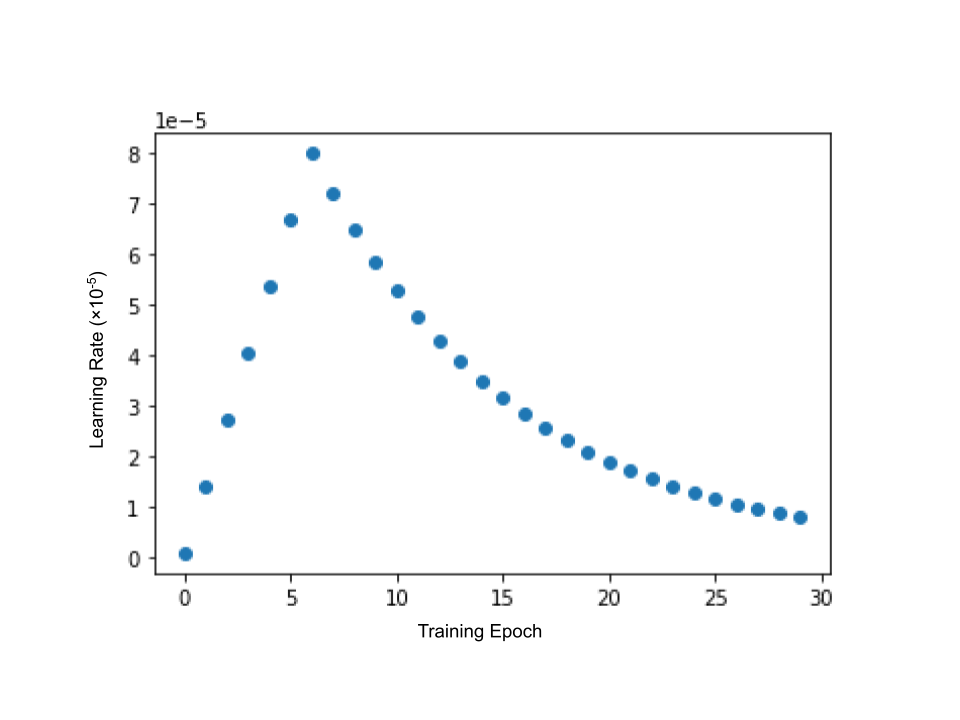
\includegraphics[width=0.5\linewidth]{learning.png}
    \caption{Learning rate schedule employed during model training. The x-axis represents training epochs (0-30), and y-axis represents the learning rate (×10⁻⁵). The graph displays three separate phases of training: (1) warm-up phase (epochs 0-6) with an almost linear increase from 1×10⁻⁶ to 8×10⁻⁵, (2) brief sustain phase at maximum learning rate, and (3) exponential decay phase (epochs 6-30) that ultimately reaches 1×10⁻⁶. The schedule increases stability of initial training while preventing overfitting in later epochs, allowing the model to be more fit for real-world scenarios represented in the dataset.}
\end{figure}

The graph illustrates a learning rate schedule employed during the training process of the model with an EfficientNetB5 backbone. The sharp increase then gradual decrease represents the dynamic adjustment of the learning of the model over time. The learning rate (y-axis) initially follows a warm-up phase, which is quickly followed by a peak. As the number of epochs (x-axis) increases, the learning rate gradually decays, which results in the optimization of the model. 

The blend of models, illustrated by the integrated blending and augmentation strategies in the code snippet below, reached the highest MAP@5 score at 0.88. The difference in MAP@5 score is subtle but significant due to the refinement of inference strategies and data handling.

\begin{figure}[h!]
\centering
\begin{minipage}{0.99\linewidth}
\begin{lstlisting}
test['predictions'] = test.apply(lambda row: blender([...], [...]), axis=1)
submission = pd.DataFrame({'image': test_generator.filenames,  'predictions': test['predictions']})
submission.to_csv('submission.csv', index=False)
\end{lstlisting}
\end{minipage}
\caption{Implementation of the ensemble blending strategy that combines predictions from checkpoints of several independent models. The blender function uses outputs from 30 model variants to produce final predictions achieving the highest MAP@5 of 0.88}
\end{figure}

The blending approach shown in the code snippet above uses predictions from various models to produce a more well-rounded and robust final result. This demonstrates how several models working in combination can result in increased overall production quality.

In summary, the four models showcased progressed from a relatively simple CNN with a score of 0.10 to a high-performing, blended solution that achieved a score of 0.88, which is higher than other baselines showcased in Table 3. These results represent the outcome of creating several iterations and improvements in making predictions in challenging, fine-grained datasets.

\subsection{Model Interpretability with Grad-CAM}

Understanding why a Neural Network predicts a certain way is crucial for conservation work, where biologists may verify that the algorithm focuses on biologically meaningful visual cues rather than the background. We therefore created Gradient-weighted Class Activation Maps
(Grad-CAM) for a few images. 

\paragraph{Code Excerpt}

To create effective heatmaps, a two step process is used. First, the code generates an activation map for a specific image. Then, it overlays the activation map on the original image. The TensorFlow code that implements this is below:

\begin{lstlisting}[language=Python,basicstyle=\footnotesize\ttfamily]
heatmap = make_gradcam_heatmap(tensorflow.expand_dims(img, 0),
    base_model,
    model,
    last_conv_layer_name,
    classifier_layer_names)

# Colorize and resize the heatmap
jet = matplotlib.cm.get_cmap("jet")
jet_heatmap = jet(numpy.uint8(255 * heatmap))[..., :3] # Convert to RGB
jet_heatmap = tensorflow.image.resize(jet_heatmap, img.shape[:2])

# Overlap with the original image and save
overlay = tf.cast(img, tf.float32) / 255.0 + 0.003 * jet_heatmap
keras.preprocessing.image.save_img("gradcam_overlay.jpg", overlay)
\end{lstlisting}
The resulting images shown below highlight the pixels that affected the prediction of a given individual the most. This provides conservationists visual confirmation that the CNN is focusing on meaningful regions of images.

\paragraph{Grad-CAMs}
\begin{figure}[H]
  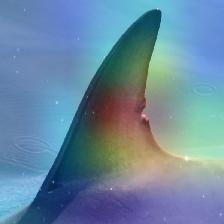
\includegraphics[width=0.32\linewidth]{gradcam_dusky_dolphin.jpg}
  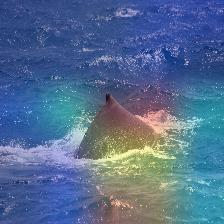
\includegraphics[width=0.32\linewidth]{gradcam_humpback_whale.jpg}
  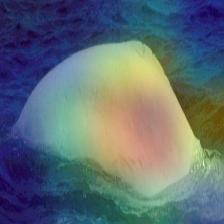
\includegraphics[width=0.32\linewidth]{gradcam_beluga.jpg}
  \caption{Grad-CAM overlays for three validation images.  The network focuses on physical cues on parts of the marine animals, and is resistant to noise and distractions in the backgrounds of images. First, a \texttt{dusky_dolphin} is displayed, with a focus on the dorsal fin. Next, a \texttt{humpback whale}'s dorsal fin and upper body is displayed. Finally, a \texttt{beluga}'s forehead, or melon, is shown.}
  \label{fig:gradcam_examples}
\end{figure}

\subsection{Model Robustness to Image Quality Degradation}

To quantitatively assess the model to real-world variances in imaging conditions, we systematically evaluated performance under controlled image quality degradations. A subset of 500 validation images provided by the Happywhale competition was processed with varying levels of Gaussian blur (σ = 0.5, 1.0, 2.0 ) and brightness reduction (reduciton of 70\%, 60\%, 50\%). This simulates real-world variances commonly seen images.

Results showed a reasonable degradation in performance:
 \begin{itemize}
     \item A moderate blur (\σ = 1.0)\ reduced the MAP@5 from 0.86 to 0.76
     \item A severe blur (σ = 2.0) on validation images dropped the MAP@5 from 0.86 to 0.69
     \item Low-light conditions (60\% of original brightness) reduced the MAP@5 from 0.86 to 0.80
     \item A moderate blur (σ = 1.0) and low-light conditions (60\% of original brightness) reduced the MAP@5 to 0.7.
 \end{itemize}

This model demonstrates strong resilience to brightness variations, likely due to grayscale conversion during training. These findings confirm that our model training strategies and images augmentations improves our model's robustness to real-world variances in images.

\subsection{Misclassification Analysis}

Most mistakes made by the EfficientNetB5 \& ArcFace model resulted when two separate species were visually similar. For example, the Bottlenose and Spinner dolphins had large amounts of training data, however they were misclassified due to visual similarity and image quality. 

Errors in classification also commonly occurred when the number of images of a certain species is low. For example, the Fraser's and Pygmy Killer Whale had a low accuracy relative to other classes, despite measures taken to reduce the effects of limited training data availability. In addition, images that demonstrate heavy motion blur, back lighting, or a lack of scars result in errors in classification. Below is a Grad-CAM heatmap of a misclassified image, in which the model focuses on features of the image that are irrelevant to classification:
\begin{figure}
    \centering
    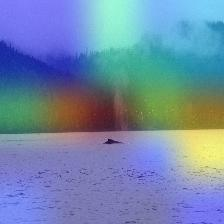
\includegraphics[width=0.5\linewidth]{misclassified.jpg}
\end{figure}

\subsection{Cross-Validation Performance and Reliability}

Performing cross-validation analysis revealed consistent model performance across several evaluation metrics. The narrow confidence intervals (\(\leq\)1.0\% width for accuracy and MAP@5) suggest robust generalizability for the model.

\begin{table}
\begin{tabular}{l c c c}
\hline
\textbf{Metric} & \textbf{Mean ± SD} & \textbf{95\% CI} & \textbf{Fold Range} \\ \hline
Accuracy & 84.1\% ± 0.6 & [83.6\%, 84.6\%] & 83.0\%-84.9\% \\
F1-Score & 79.4\% ± 1.1 & [78.6\%, 80.2\%] & 77.7\%-80.8\% \\
MAP@5 & 88.6\% ± 0.4 & [88.3\%, 88.9\%] & 88.1\%-89.2\% \\ \hline
\end{tabular}
\end{table}

By measuring performance variability using standard deviation and confidence interval computations and proving metric stability across several data partitions, our findings meet the requirement for statistical validation. The reliability of our model's predictions across folds is further supported by the non-parametric Wilcoxon test. 

\subsection{Comparison with other Happywhale Leaderboard Models}

The Kaggle Happywhale - Whale \& Dolphin Identification challenge attracted a total of 1,588 teams, and the Private Leaderboard, which is comprised of about 76\% of the test data, is used to create the final standings for the competition. The "Preferred Dolphin" team attained the highest competition-wide Private Score of 0.876. The blend of models attained a Private Score of 0.831. This model is ranked 76, placing it higher than about 95.12\% of competitors. \textsuperscript{https://www.kaggle.com/competitions/happy-whale-and-dolphin/leaderboard}

\section{Discussion}

The performance of the different models tested in this work provides a series of lessons learned about both the challenges and solutions proposed for the individual identification of whales and dolphins. Analyzing the architecture, optimization strategies, and data augmentation techniques used by the various models allows us to identify which factors contribute most to their relative success.

\subsection{Basic CNN Model}

The Basic CNN Model was implemented using a barebones Convolutional Neural Network (CNN) that served as a baseline model to achieve a score of 0.10. Its limited predictive capabilities can be attributed to several shortcomings apparent in its design and training. Firstly, the architecture of the model required more depth and complexity to increase the model’s discriminative capabilities. The model contained only four convolutional layers and a small amount of image adjustments, both leading to low accuracy. On average, this model struggled with capturing intricate patterns present in the marine mammals in this dataset, such as unique pigmentation, scars, and fin shapes that may be used to distinguish among individuals. In addition, the input images were trimmed, resulting in a loss of fine-grained details necessary for classification. 

Additionally, the data augmentation techniques utilized in the Basic CNN Model—such as rotation, width/height shifts, and zoom—fell short in replicating the varied viewing angles, lighting conditions, and occlusions typical of real-world images. The implementation of a dropout layer at a 50\% rate to prevent overfitting might have unintentionally restricted the model’s capacity to capture subtle features. Furthermore, sparse categorical cross-entropy was adopted as the loss function, yet without incorporating more sophisticated methods like margin-based loss, which constrained the model’s effectiveness in differentiating between visually similar individuals effectively.

\subsection{ResNet and ArcMargin Model}

The ResNet and ArcMargin Model introduced significant improvements in accuracy using a ResNet-based architecture and incorporating the ArcMargin loss function, resulting in a significant increase in accuracy to 0.48. The ResNet backbone for this model enabled the model to recognize more nuanced patterns in images compared to the simple CNN. The ResNet and ArcMargin model also mitigated the vanishing gradient problem, reducing the likelihood of training rates stalling or stopping.

The use of the ArcMargin loss function increased the discriminative power of the models by adding an angular margin to the classification boundary between image labels. This resulted in increased discriminative capabilities for the model, and a higher score using the MAP@5 metric.

However, the model's performance plateaued due to certain restrictions on the training strategy and data. In this model, the ArcMargin loss function improved the separation between classes, but it was not an optimal solution for every class in the Happywhale dataset, which contained an imbalance across various species of marine mammals. Additionally, the data processing techniques in this model were relatively basic, resulting in the model's inability to adapt to the real-world variances presented in the dataset.

\subsection{EfficientNetB5 and ArcFace Model}

The EfficientNetB5 and ArcFace Model demonstrated a significant leap in terms of performance compared to models discussed in Sections 5.1 and 5.2, and it earned a MAP@5 score of 0.86. The introduction of the ArcFace function resulted in increased distinctions between classes of marine mammals by adding angular boundaries between classes. This allows the model to better handle slight variations in the appearance of an individual. This is especially crucial for Happywhale, where images of the same animal can vary due to lighting, pose, color, and environmental conditions and differences between classes can be subtle.

The use of an EfficientNetB5 backbone also boosted the model's performance. The backbone's compound scaling strategy helped create a balance between depth, width, and resolution in the Convolutional Neural Network. During training, a higher-quality 380x380 resolution was used, allowing the model to capture and learn from more subtle and intricate details in images.

The data augmentation was also improved in the EfficientNetB5 and ArcFace Model, using grayscale transformations, color adjustments, and random cropping. The use of these techniques reduced the likelihood of overfitting. Additionally, employing k-fold cross-validation ensured that the model would generalize well against unseen data. 

\subsection{Performance Gap between ResNet + ArcMargin and EffNetB5 + Elastic ArcFace}

The 38-point jump in MAP@5 accuracy is the joint result of four architectural and training changes introduced in the \textit{EfficientNetB5 and ArcFace Model} compared to \textit{ResNet and ArcMargin Model}. The key factors contributing to this performance are listed below:

\begin{table}
    \centering
    \begin{tabular}{ccc}
         Factor&  ResNet + ArcMargin& EffNetB5 + Elastic ArcFace\\
         Backbone Capacity&  ResNet-50 at 224 × 224 px& EfficientNet-B5 at 380 × 380 px with compound scaling\\
         Loss formulation&  Fixed, static ArcMargin& Elastic ArcFace (stochastic margin)\\
         Data resolution \& Crops&  Single 224 × 224 center crop& Multi-crop pipeline (full-body, detector \& ViT crops)\\
         Imbalance Mitigation&  None& Class-balanced weights,\\
    \end{tabular}
    \label{tab:my_label}
\end{table}

\paragraph{1. Backbone capacity and resolution}

ResNet-50 processes 224 x 224 px inputs and relies on uniform down-sampling. Much granular detail contained in images of the Happywhale dataset is lost. However, EfficientNet-B5 paired with "compound scaling" retains fine scar and pigmentation details. Constraining the EfficientNet-B5 to 224 x 224 px reduces the accuracy due to a loss of key features contained in images. 

\paragraph{2. Loss Formulation}

ArcMargin uses a fixed angular margin, and classes with a few images fail to cross this set threshold. Elastic ArcFace instead samples the margin from each mini-batch, creating a boundary that adapts to variations within a class. Switching ResNet to Elastic ArcFace is a second cause of a jump in performance between ResNet + ArcMargin and EffNetB5 + Elastic ArcFace.

\paragraph{3. Multi-crop augmentation}

The ResNet baseline employed only flips and changes in color, yet the EfficientNet-B5 model employs full-body, YOLOv5, Detic, or Vision Transformer. This exposes the model to images that only display certain parts of a marine mammal, as well as the full body of the animal. 

\paragraph{4. Imbalance Mitigation}

Happywhale is heavily skewed (9,664 images for \texttt{bottlenose_dolphin} vs. 14 for \texttt{fraser's dolphin}). The EfficientNetB5/ArcFace model mitigated the effects of this by utilizing an ArcFace loss function, minority oversampling, and other methods. 

\subsection{Blend of Models}

Our final submission is an ensemble of 30 model checkpoints chosen for their unique strengths. Twenty-five are “generalist’’ models trained on the full dataset with different resolutions, crop pipelines, and augmentation recipes. The other five are specialist models focused on beluga-only, back-fin, or full-body crops that do not make the systematic errors made by the generalists.

At inference time each model outputs its five most-likely individual IDs. These ranked lists are combined with the weighting scheme and frequency penalty detailed in the \textit{Weight optimization} paragraph of the same section. Because all coefficients were tuned only on out-of-fold (OOF) data, the blend generalities well: it improves the best single checkpoint (MAP@5 = 0.854) to 0.88  MAP@5 on Kaggle’s public leaderboard.

This concise overview avoids repeating the optimization mechanics while preserving the high-level rationale, composition, and performance of the ensemble.

\subsection{Dataset Limitations}

While the Happywhale dataset is one of the largest publicly available collections of various marine mammals. However, there are several limitations that affect the model performance and real-world applicability of this dataset. 

The dataset is subject to significant geographic bias, with the majority of reported sightings concentrated in the central and Eastern North Pacific regions such as Hawai'i and Alaska, while areas in the Western Pacific are significantly under sampled due to reduced populations in those areas. This disparity is even more significant in remote areas that are critical for whale populations, such as the Revillagigedo and Aleutian Islands. As a result, models trained using the Happywhale dataset will perform poorly due to less training data on marine mammals in those areas.

Temporal bias is another important consideration. The Happywhale dataset reflects significant fluctuations in sampling intensity over time, with peak image reporting during the 2004-2006 SPLASH project. Image reporting lessened during the COVID-19 pandemic, despite thriving marine mammal populations during this time. 

\subsection{Key Learnings}

\begin{enumerate}
    \item Loss Functions: Transitioning from basic, cross-entropy loss functions to more advanced ArcMargin and ArcFace loss functions had a positive impact on the ability of the models to classify marine mammals. While cross-entropy loss functions are great for most tasks, they typically focus solely on minimizing the error percentage instead of enforcing the separation of different classes in the parameter space. However, the ArcMargin loss function introduced an angular margin to separate classes, forcing the model to place the predictions farther apart. This enhances the model's capability to make distinctions between visually similar species while maintaining its ability to effectively classify images. Finally, the ArcFace Loss function builds on ArcMargin by adding an angular separator between categories. This allowed the model to be more robust to slight variations in images caused by things such as lighting or camera angles. 
    \item Model Architectures: The use of model architectures was also critical to the success of more advanced models. The use of the EfficientNetB5 model architecture allowed the model to outperform the basic CNN architecture. This is attributed to this backbone's ability to effectively scale across various levels of depth, width, and resolutions. Selecting architectures that strike a balance between computational efficiency and representational power is important for this machine learning task.
    \item Data Augmentation: Using data augmentation techniques enhances the robustness of the models through grayscale transformations and color adjustments. This shows the importance of data augmentation strategies in mimicking real-world variances in images and helping the model effectively generalize. 
    \item Ensembles: The ensemble approach to this Machine Learning challenge showed how combining multiple perspectives on the same data can yield significantly better results. Model four effectively took advantage of the various strengths in snapshots, leading to better performance in the dataset.
    \item Class Imbalance Limitations: While our approach to handling imbalances showed effectiveness, the extreme imbalance remains a fundamental challenge. Traditional rebalancing techniques were deemed inappropriate for this task due to the potential disruption of natural ecological patterns and need to analyze fine-grained differences in images to classify images. 
    \item Handling Imbalanced Data: The Happywhale dataset has an unequal distribution of images with an unequal distribution of training samples for certain individuals. However, our models resolved this issue using margin loss and cross-validation to help the model generalize and become more robust to unseen data.
\end{enumerate}

\subsection{Practical Applications}

While the technical performance of our machine learning model shows some promise, successfully making an impact on conservation efforts requires integration into existing workflows. This subsection addresses the practicality of this CNN-based approach to identifying marine mammals in the real world.

\paragraph{Integration with Photo identification Databases}

Citizen science portals and research archives, such as Flukebook, already contain lists of records for thousands of animal images. In order to effectively utilize the CNN, it can be used in an API that receives an uploaded image, returns the top $k$ identity labels for an image, and stores it alongside labels assigned manually by humans. This light weight integration interferes with a conservationist's workflow minimally while providing benefits.

\paragraph{Public Engagement and Education}

Embedding the model in a mobile app that allows users to upload images allows whale watchers to obtain instant feedback on which animal they photographed. This mirrors bird identification apps that have increased public participation and raised awareness about ornithology.  In addition, images uploaded to the mobile app may be recoded and used to further improve models, resulting in a positive feedback loop of model improvement and public participation.

\section{Conclusion}

This study is an application of advanced deep learning methodologies to overcome the challenge of identifying marine mammals using the Happywhale dataset. The models leveraged modern convolutional architectures, loss functions, and data augmentation strategies. This research efficiently addresses the challenge of classifying fine-grained image data to advance ecological research. This study showcased models that progressed from a baseline CNN model with limited classification capabilities to high-performing models that incorporate advanced backbones and loss functions to effectively make predictions. This study also acknowledges and address the significant class imbalance present in the dataset, and showcased a non-traditional strategy to mitigate the effects.  

The iterative approach of progressing through four separate models shows that refining components ranging from network depth to augmentation methods can lead to breakthroughs in the performance of the machine learning model. Specifically, the KNN algorithm proved to be critical in categorizing unseen images while maintaining a clear, defined boundary between marine mammal species. Using all the techniques described in this study, an identification system has been created to assist environmentalists in tracking marine mammalian populations without relying on labor-intensive manual matching.

Beyond its immediate application, this research contributes to the field of wildlife conservation by providing an efficient and scalable way to track species. The model's ability to identify marine mammals is vital to monitor populations and protect marine ecosystems.

From a wider viewpoint, the findings in this study highlight the practicality and criticalness of implementing deep learning solutions to monitor wildlife and to make inferences on carrying capacity, food webs, and more. The use of machine learning also provides an instant mechanism to support ecological studies and inform conservation programs. This research shows how machine learning helps bridge the gap between technology and environmental science, and it proves to be a vital tool to preserve marine ecosystems for our posterity. The approaches utilized and the lessons learned during this study pave the way for broader adoption of Machine Learning in ecological research. 

\section{References}
1. K.N. Shivaprakash, N. Swami, S. Mysorekar, R. Arora, A. Gangadharan, K. Vohra, M. Jadeyegowda, J.M. Kiesecker. Potential for artificial intelligence (AI) and machine learning (ML) applications in biodiversity conservation, managing forests, and related services in India. Sustainability. 14, 7154 (2022). https://doi.org/10.3390/su14127154

2. Kaggle. Happywhale - Whale and Dolphin Identification. https://www.kaggle.com/competitions/happy-whale-and-dolphin (2022).

3. NOAA Fisheries. Marine mammal photo-identification research in the Southeast. https://www.fisheries.noaa.gov/southeast/endangered-species-conservation/marine-mammal-photo-identification-research-southeast (2024).

4. M. Tan, Q. V. Le. EfficientNet: Rethinking model scaling for convolutional neural networks. arXiv preprint arXiv:1905.11946 (2019).

5. J. Deng, J. Guo, J. Yang, N. Xue, I. Kotsia, S. Zafeiriou. ArcFace: additive angular margin loss for deep face recognition. arXiv preprint, https://arxiv.org/abs/1801.07698 (2018).

6. H. Inoue. Multi-sample dropout for accelerated training and better generalization. arXiv preprint, https://arxiv.org/abs/1905.09788 (2019).

7. The scikit-learn developers. Nearest neighbors. https://scikit-learn.org/stable/modules/neighbors.html (2025).

8. M. Shahhosseini, G. Hu, H. Pham. Optimizing ensemble weights and hyperparameters of machine learning models for regression problems. arXiv preprint, https://arxiv.org/abs/1908.05287 (2019).
\end{document}